\section{Tree Decompositions And Treewidth}
\begin{definition}\label{8.1}
    A \textbf{tree decomposition}\index{tree decomposition} of a graph $G=(V,E)$ is a pair $D=(S,T)$, where $S=\{{\color{cyan}{X_i}}:i\in {\color{blue}{I}}\}$ is a set of subsets of $V$ and $T=({\color{blue}I},{\color{red}F})$ is a tree such that the following hold:
    \begin{enumerate}
        \item $\bigcup_{i\in I}X_i=V$;
        \item For every edge $\{u,v\}\in E$, there is an $i\in I$ such that $u,v\in X_i$;
        \item For all $v\in V$, the subtree of $T$ induced by $\{i\in I:v\in X_i\}$ is connected;
    \end{enumerate}
The sets $X_i$ are called \textbf{bags}\index{bag}.\\
The \textbf{width} of  $D$ is $wd(D)=\max_{i\in I}|X_i|-1$.\\
The \textbf{treewidth}\index{treewidth} of $G$ is $tw(G)=\min\{wd(D):D\text{ is a tree decomposition of }G\}$. 

 \begin{center}
            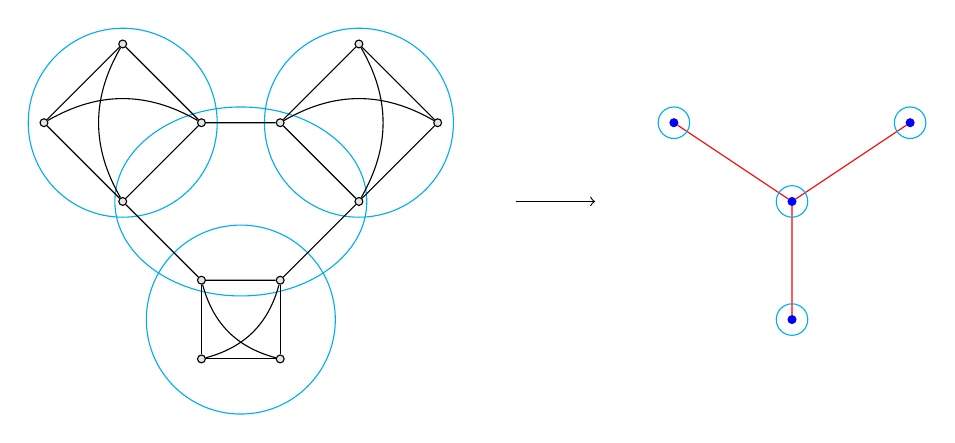
\begin{tikzpicture}[
            vertex/.style={circle, draw, fill=gray!20, minimum size=1mm, inner sep=0pt}
            ]
            \node[vertex] (a) at (0,1) {};
            \node[vertex] (b) at (1,2) {};
            \node[vertex] (c) at (1,0) {};
            \node[vertex] (d) at (2,1) {};
            \node[vertex] (e) at (2,-1) {};
            \node[vertex] (f) at (2,-2) {};
            \node[vertex] (g) at (3,1) {};
            \node[vertex] (h) at (3,-1) {};
            \node[vertex] (i) at (3,-2) {};
            \node[vertex] (j) at (4,2) {};
            \node[vertex] (k) at (4,0) {};
            \node[vertex] (l) at (5,1) {};
            %\node[vertex, blue] (m) at (1,1) {};
            %\node[vertex, blue] (n) at (2.5,0) {};
            %\node[vertex, blue] (o) at (2.5,-1.5) {};
            %\node[vertex, blue] (p) at (4,1) {};
            
            \draw[cyan] (1,1) circle (1.2cm);
            \draw[cyan] (2.5,0) ellipse (1.6cm and 1.2cm);    
            \draw[cyan] (2.5,-1.5) circle (1.2cm);
            \draw[cyan] (4,1) circle (1.2cm);

            \draw (a) -- (b) -- (d) -- (g) -- (j) -- (l);
            \draw (a) -- (c) -- (e) -- (h) -- (k) -- (l);
            \draw (c) -- (d);
            \draw (g) -- (k);
            \draw (e) -- (f) -- (i) -- (h);
            \draw (a) to[bend left] (d);
            \draw (b) to[bend right] (c);
            \draw (e) to[bend right] (i);
            \draw (f) to[bend right] (h);
            \draw (g) to[bend left] (l);
            \draw (j) to[bend left] (k);
            %\draw[red] (m) -- (n) -- (o);
            %\draw[red] (n) -- (p);

            
            \node[vertex, blue] (q) at (8,1) {};
            \node[vertex, blue] (r) at (9.5,0) {};
            \node[vertex, blue] (s) at (9.5,-1.5) {};
            \node[vertex, blue] (t) at (11,1) {};

            \draw[red] (q) -- (r) -- (s);
            \draw[red] (r) -- (t);

            \draw[cyan] (q) circle (0.2 cm);
            \draw[cyan] (r) circle (0.2 cm);
            \draw[cyan] (s) circle (0.2 cm);
            \draw[cyan] (t) circle (0.2 cm);
            
            \draw[->] (6,0) -- (7,0);


            \end{tikzpicture}
    \end{center}

\end{definition}
\begin{remark}\label{8.2}
    Every graph has a trivial tree decomposition of width $|V(G)|-1$, which has a single bag containing all vertices of $G$.
\end{remark}
\begin{remark}\label{8.3}
    Equivalent formulations for $(iii)$:
    \begin{itemize}
        \item [(iii')] If, for $v\in V$, we have $v\in X_i$ and $v\in X_j$, then $v\in X_k$ for all $k\in I$ that lie on the unique path from $i$ to $j$ in $T$.
        \item [(iii'')] For $i,j\in I$ and $k\in I$ on the unique path from $i$ to $j$, $X_i\cap X_j\subseteq X_k$.
    \end{itemize}
    Since the treewidth of a graph $G$ is the maximum of the treewidths of its connected components, we will focus on connected graphs. We have $G=K_1\iff tw(G)=0$, we assume $|V(G)|\geq 2$ from now on.
\end{remark}
\begin{lemma}\label{8.4}
    Let $G$ be a connected graph with tree decomposition $D=(S,T)$. For every clique $C\subseteq V(G)$, there exists a bag $X_i$, with $C\subseteq X_i$.
\end{lemma}
\begin{proof}
    Induction on $k=|C|$. For $k=1$, this is $(i)$, for $K=2$ it's $(ii)$ (Definition \ref{8.1}).\\
    Now let $k\geq 3$ and let $u,v,w$ be distinct vertices in $C$. By IH, there exist bags $X_a,X_b,X_c$ s.t. $C\setminus\{u\}\subseteq X_a,\quad C\setminus\{v\}\subseteq X_b,\quad C\setminus\{w\}\subseteq X_c$. If any two of $a,b,c$ are equal, the corresponding bag contains $C$. Thus let $a,b,c$ be pairwise distinct. Let $P_{ab},P_{ac},P_{bc}$ be the unique paths between $ab,ac,bc$ in $T$. They must share a vertex $d\notin\{a,b,c\}$ since concaterating $P_{ab},P_{ac},P_{bc}$ would be a cycle otherwise, but $T$ is a tree.
     \begin{center}
            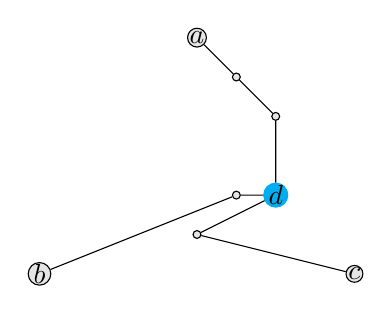
\begin{tikzpicture}[
            vertex/.style={circle, draw, fill=gray!20, minimum size=1mm, inner sep=0pt}
            ]
            \node[vertex] (a) at (0,3) {$a$};
            \node[vertex] (b) at (-2,0) {$b$};
            \node[vertex] (c) at (2,0) {$c$};
            \node[vertex, cyan] (d) at (1,1) {\color{black}$d$};
            \node[vertex] (e) at (0,0.5) {};
            \node[vertex] (f) at (1,2) {};
            \node[vertex] (g) at (0.5,2.5) {};
            \node[vertex] (h) at (0.5,1) {};

            \draw (a)--(g)--(f)--(d)--(e)--(c);
            \draw (b)--(h)--(d);
            
            \end{tikzpicture}
    \end{center}
    By $(iii'')$ from \ref{8.3}, we have $C\setminus\{u,v\}\subseteq X_a\cap X_b\subseteq X_d$.\\
    Similarly, $C\setminus\{u,w\}\subseteq X_d$ and $C\setminus\{v,w\}\subseteq X_d\implies C\subseteq X_d$.
\end{proof}
\begin{corollary}\label{8.5}
    For every graph $G$, we have $\omega(G)-1\leq tw(G)$.
\end{corollary}
\begin{lemma}\label{8.6}
    If $H$ is a minor of $G$, then $tw(H)\leq tw(G)$
\end{lemma}
\begin{proof}
    If $H$ is obtained from $G$ by deleting a vertex or an edge, then $tw(H)\leq tw(G)$ as every tree decomposition of $G$ remains one for $H$ (after deleting the vertex/vertices from all bags containing them).\\
    Suppose $H$ is obtained from $G$ by contracting an edge $\{u,v\}$.\\
    Let $D=(S,T)$ be a tree decomposition of $G$. Replace all occurences of $u$ and $v$ in the bags by a new vertex $w$. Since bags containing $u$ induce a subtree of $T$, similarly for $v$, and there is a bag containing $u$ and $v$, the bag containing $w$ induces a subtree in $T$ as well.
\end{proof}
\begin{lemma}\label{8.7}
    Let $G=(V,E)$ connected with $|V|\geq 2$. Then $tw(G)=1\iff G$ is a tree.
\end{lemma}
\begin{proof}
    "$\impliedby$"\\
    Let $G$ be a tree. Choose $s\in V$ and run DFS (Depth-First Search) on $G$. This yields for every $v\in V\setminus\{s\}$ a unique predecessor $\pi(v)$.\\
    Set $X_s=\{s\}$, $X_v=\{v,\pi(v)\}$ $\forall v\in V\setminus\{s\}$, $T=G$, $S=\{X_v:v\in V\}$.\\
    We claim that $D=(T,S)$ is a treedecomposition of $G$.\\
    Properties (i) and (ii) directly follow from the constructions. For $v\in V$, the set of bags containing $v$ is $X_v$ together with all $X_w$ where $w$ is a child of $v$. Thus the subtree induced by the corresponding vertices in $T$ is connected. $\implies tw(G)=1$ (bags only have a max. of $2$ vertices in them).
     
 \begin{center}
            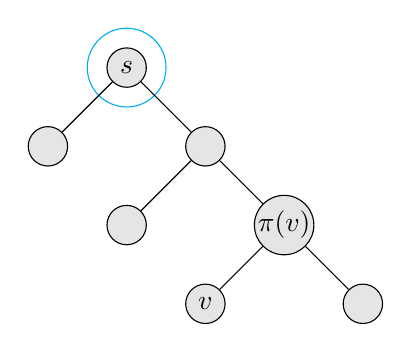
\begin{tikzpicture}[
            vertex/.style={circle, draw, fill=gray!20, minimum size=5mm, inner sep=0pt}
            ]
            \node[vertex] (a) at (0,7) {$s$};
            \node[vertex] (b) at (-1,6) {};
            \node[vertex] (c) at (1,6) {};
            \node[vertex] (d) at (0,5) {};
            \node[vertex] (e) at (2,5) {$\pi(v)$};
            \node[vertex] (f) at (1,4) {$v$};
            \node[vertex] (g) at (3,4) {};
            
            \draw[cyan] (a) circle (0.5cm);
            \drawellipse[cyan, thick]{a}{b}{0.5cm}{0.7cm}
            \drawellipse[cyan, thick]{a}{c}{0.5cm}{0.7cm}
            \drawellipse[cyan, thick]{c}{d}{0.5cm}{0.7cm}
            \drawellipse[cyan, thick]{c}{e}{0.5cm}{0.7cm}
            \drawellipse[cyan, thick]{e}{f}{0.5cm}{0.7cm}
            \drawellipse[cyan, thick]{e}{g}{0.5cm}{0.7cm}
            \draw (a)--(b);
            \draw (a)--(c)--(d);
            \draw (c)--(e)--(f);
            \draw (e)--(g);
        


            \end{tikzpicture}
    \end{center}
    "$\implies$"\\
    If $G$ is not a tree $\implies$ $G$ contains a cycle and hence a $K_3$ minor. By Corollary \ref{8.5}, we have $tw(K_3)=2$ and by Lemma \ref{8.6}, $2=tw(K_3)\leq tw(G)\lightning\implies G$ is a tree.
\end{proof}
\begin{remark*}
    Computing treewidth is NP-hard
\end{remark*}
\begin{theorem}[Bodlaender]\label{8.8}
    There exists an algorithm that, given a graph $G$ with $tw(G)=k$, computes a tree decomposition of $G$ of width $k$ in time: $2^{o(k^3)}|V(G)|$
\end{theorem}
\begin{remark*}
    \begin{itemize}
        \item Bodlaender et al. (2016): An algorithm that constructs a treedecomposition of width $\leq 5k+4$ or decides $tw(G)\geq k$ in $o(2^{o(k)}n)$
        \item Korhonen (2021): width $\leq 2k+1$ with same runtime
        \item Korhonen, Lokshtanov (2023): width $k$, runtime $2^{o(k^2)}o(n^4)$
        \item open question: What is the complexity of computing treewidth on planar graphs. Is it in P?
    \end{itemize}
\end{remark*}
\begin{definition}\label{8.9}
    A \textbf{nice treedecomposition}\index{nice treedecomposition} $D=(S,T)$ of a graph $G=(V,E)$ is a tree decomposition in which a root vertex can be choosen s.t. $T$ is a binary tree (i.e. every vertex has at most $2$ children) and such that every vertex of $T$ is of one of the following types:
    \begin{itemize}
        \item \textbf{leaf}: if $i\in V(T)$ is a leaf of $T$, then $|X_i|=1$
        \item \textbf{introduce node}: if $i\in V(T)$ has exactly one child $j$ and $X_i=X_j\cap\{v\}$ for some $v\in V(G)$
        \item \textbf{forget node}: if $i\in V(T)$ has exactly one child $j$ and $X_i=X_j\setminus\{v\}$ for some $v\in X_j$
        \item \textbf{join node}: if $i\in V(T)$ has precisely two children $j_1,j_2$ and $X_i=X_{j_1}=X_{j_2}$
    \end{itemize}
\end{definition}
\begin{theorem}\label{8.10}
    Let $D=(S,T)$ a tree decomposition of $G=(V,E)$. Then we can construct a nice treedecomposition $D'=(S',T')$ of $G$ with $tw(D')\leq tw(D)$, $|V(T')|\leq c tw(D)|V(T)|$ in polynomial time.
\end{theorem}
\begin{proof}
    Root $T$ at an arbitrary vertex $s\in V(T)$.
    \begin{enumerate}
        \item Make $T$ binary:\\
        For every $i\in V(T)$ that has $\geq 3$ children $j_1,...,j_t$, replace $i$ and its descendants as follows:
        \begin{center}
            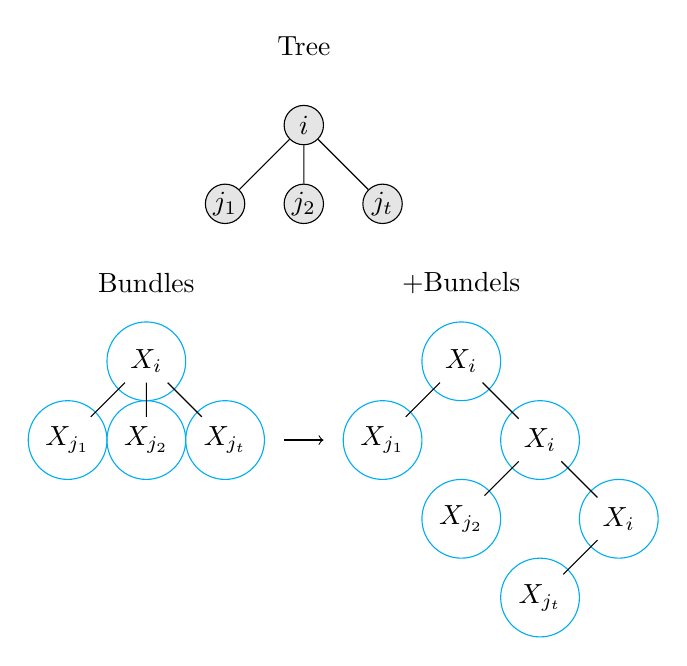
\begin{tikzpicture}[
            vertex/.style={circle, draw, fill=gray!20, minimum size=5mm, inner sep=0pt}
            ]
            \node at (0,9) {Tree};
            \node[vertex] (a) at (0,8) {$i$};
            \node[vertex] (b) at (-1,7) {$j_1$};
            \node[vertex] (c) at (0,7) {$j_2$};
            \node[vertex] (d) at (1,7) {$j_t$};
            
            \node at (-2,6) {Bundles};
            \node (e) at (-2,5) {$X_i$};
            \node (g) at (-3,4) {$X_{j_1}$};
            \node (h) at (-2,4) {$X_{j_2}$};
            \node (i) at (-1,4) {$X_{j_t}$};
            
            \node at (2,6) {+Bundels};
            \node (j) at (2,5) {$X_i$};
            \node (k) at (1,4) {$X_{j_1}$};
            \node (l) at (3,4) {$X_i$};
            \node (m) at (2,3) {$X_{j_2}$};
            \node (n) at (4,3) {$X_i$};
            \node (o) at (3,2) {$X_{j_t}$};

            
            \draw[cyan] (e) circle (0.5cm);
            \draw[cyan] (g) circle (0.5cm);
            \draw[cyan] (h) circle (0.5cm);
            \draw[cyan] (i) circle (0.5cm);
            \draw[cyan] (j) circle (0.5cm);
            \draw[cyan] (k) circle (0.5cm);
            \draw[cyan] (l) circle (0.5cm);
            \draw[cyan] (m) circle (0.5cm);
            \draw[cyan] (n) circle (0.5cm);
            \draw[cyan] (o) circle (0.5cm);

            \draw (b)--(a)--(c);
            \draw (a)--(d);
            \draw (g)--(e)--(h);
            \draw (e)--(i);
            \draw (k)--(j)--(l)--(m);
            \draw (l)--(n)--(o);
        
            \draw[->] (-0.25,4) -- (0.25,4);

            \end{tikzpicture}
    \end{center}
    \item Make all vertices with precisely two children join nodes:
    \begin{center}
            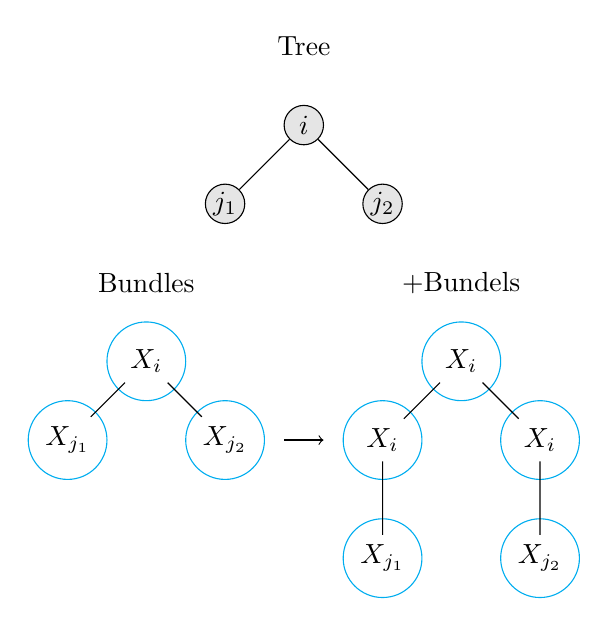
\begin{tikzpicture}[
            vertex/.style={circle, draw, fill=gray!20, minimum size=5mm, inner sep=0pt}
            ]
            \node at (0,9) {Tree};
            \node[vertex] (a) at (0,8) {$i$};
            \node[vertex] (b) at (-1,7) {$j_1$};
            \node[vertex] (d) at (1,7) {$j_2$};
            
            \node at (-2,6) {Bundles};
            \node (e) at (-2,5) {$X_i$};
            \node (g) at (-3,4) {$X_{j_1}$};
            \node (i) at (-1,4) {$X_{j_2}$};
            
            \node at (2,6) {+Bundels};
            \node (j) at (2,5) {$X_i$};
            \node (k) at (1,4) {$X_i$};
            \node (l) at (3,4) {$X_i$};
            \node (m) at (1,2.5) {$X_{j_1}$};
            \node (o) at (3,2.5) {$X_{j_2}$};

            
            \draw[cyan] (e) circle (0.5cm);
            \draw[cyan] (g) circle (0.5cm);
            \draw[cyan] (i) circle (0.5cm);
            \draw[cyan] (j) circle (0.5cm);
            \draw[cyan] (k) circle (0.5cm);
            \draw[cyan] (l) circle (0.5cm);
            \draw[cyan] (m) circle (0.5cm);
            \draw[cyan] (o) circle (0.5cm);

            \draw (b)--(a)--(d);
            \draw (g)--(e)--(i);
            \draw (m)--(k)--(j)--(l)--(o);
        
            \draw[->] (-0.25,4) -- (0.25,4);

            \end{tikzpicture}
    \end{center}
    \end{enumerate}
\end{proof}